% UTF-8

% single-chapter commands
\documentclass[../main/thesis.tex]{subfiles}
\onlyinsubfile{\setcounter{chapter}{3}}  % single-chapter command
\begin{document}


\chapter{Algorithmen zur Generalisierung}

\section{Vorgehensweise}

...

% Erst über Generalisierung nachgedacht, da sie das schwierigerer Problem zu sein schien (in der Erwartung, die Identifikation ließe sich evtl. "nebenbei" lösen).
% Die Generalisierung ist auf den allerersten Blick ein einfaches geometrisches Problem, das keiner ausgefeilten Algorithmen a la 2.5 bedarf. Erst mal probiert, ob es sich so lösen lässt. Später festgestellt (-> Implementierung?), dass es in der Tat nicht so schrecklich schwierig war, jedoch die Entscheidung, was zusammengehört und was nicht, im Allgemeinen Fall schwieriger als erwartet war (ein Problem, das allerdings wohl auch für die Lösungen aus 2.5 bestanden hätte, womöglich gar in verstärktem Ausmaß).

% damals sehr früh (noch vor Anmeldung) den Algorithmus in groben Zügen aufgestellt und implementiert
% Vorgehen war im Prinzip, das Problem graphisch/geometrisch anzugehen und auf Papier zu lösen, dann in Code zu übertragen
% anschließend nur noch (sehr umfangreiche) Verbessserungen vorgenommen, insbesondere zur Flexibilisierung (individuellere Analyse, unterschiedliche Testdaten, Spezialfälle)
% zeitaufwändig: Alg. implementieren; insb.: Probleme im Workflow lösen (z. B. I/O), OOP, die Details des Alg. so hinbekommen, dass er halbwegs "rund" läuft, Probleme wie bei Kreuzungen
% habe versucht, ein wenig Test-Driven Development zu lernen, was mir schwer fiel, weil ich ständig die Struktur änderte
% erst versucht, rein geometrisch zu arbeiten, dann festgestellt (mit Jochen), dass bei Autobahnen etc Tags idR passen und die Sache erleichtern

% an dieser Stelle außerdem big picture: wie hängen die folgenden teile zusammen?
% -> lt. Themenblatt soll das Analyseergebnis auch separat von der Generalisierung zu verwenden sein!
% d.h. die Main-Klasse / Fassade sollte gar nicht hier beschrieben werden, das ist ein Implementierungsdetail (unter Kap. 5 zu beschrieben, wozu aber Kap. 5 wohl etwas umorganisiert werden müsste)
% anstatt des Analyser-Outputs ist tatsächlich bisher der CorrelationGraph das Analyseergebnis, jedoch noch unvollständig (man bräuchte noch eine Art Metrik, dass z. B. ab 80% parallelen Segmenten zwei Ways als parallel gelten; evtl. auch einen Append-Schritt, denn zur (verlangten) Identifikation paralleler Linienzüge müssten diese erst mal aus den Ways erzeugt werden, falls die Ways nicht ausreichen)

% im CLI sieht's im Moment in etwa so aus:
% 1. create OsmDataset (als InputDataset-Instanz, via ShapeReader)
% 2. Combiner.run
% 3. output
% also eigentlich nichts, was algorithmisch einer besonderen Beschreibung bedarf

% an dieser Stelle außerdem __Überleitung__: was kann man aus 2.5 für lehren/erkenntnisse ziehen? irgendwas anwendbares dabei? wenn ja, warum nicht?


%\section{Beschreibung der Algorithmen}

Im Folgenden werden die gefundenen Algorithmen zunächst in allgemeinen Begriffen beschrieben, wobei der Fokus auf ihrem Zusammenwirken und ihren Abhängigkeiten voneinander liegt.
Im Anschluss daran folgt ihre formale Beschreibung.

% erst Grundprinzip / -idee / -ansatz beschreiben, dann Edge Cases

\section{Grundprinzip}

Um das Zusammenfassen paralleler Linienzüge vorzubereiten, werden alle \term{nodes} des einen Linienzugs jeweils einem gegenüberliegenden \term{node} auf dem parallelen Linienzug zugeordnet.
Die Verbindung der Mittelpunkte zwischen den so einander zugeordneten \term{nodes} ergibt direkt den zusammengefassten Linienzug als Ergebnis der Generalisierung (Abbildung~\ref{fig:general-approach}).

Dieses Vorgehen vermeidet, dass die in Abschnitt~\ref{osm-fragmentation} besprochene häufige ungleichmäßige Fragmentierung von \osm-Linienzügen in mehrere \term{ways} einen Einfluss auf den Generalisierungsvorgang hat.
Aufgrund der nicht immer gleichen Anzahl und Verteilung der \term{nodes} kommt es vor, dass ein \term{node} des einen Linienzugs mehreren \term{nodes} des anderen Linienzugs zugeordnet wird, was jedoch unproblematisch ist.

\begin{figure}[ht]
  \begin{minipage}[t]{.5\linewidth}
    \centering
    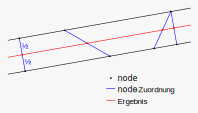
\includegraphics[width=\ScaleIfNeeded]{../chapter4/general-approach}
    \caption{general-approach}\label{fig:general-approach}
  \end{minipage}%
  \begin{minipage}[t]{.5\linewidth}
    \centering
    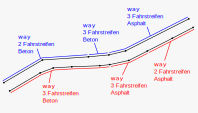
\includegraphics[width=\ScaleIfNeeded]{../chapter4/motorway-fragments}
    \caption{motorway-fragments}\label{fig:motorway-fragments}
  \end{minipage}
\end{figure}

Um zwei gegenüberliegende \term{nodes} einander zuordnen zu können, müssen zunächst die Linien, deren Teil sie sind, als zueinander parallel erkannt werden.
Auch hierbei ist die erwähnte ungleichmäßige Fragmentierung in bestimmten Fällen problematisch.
Beispielsweise müssten die einzelnen \term{ways} in Abbildung~\ref{fig:motorway-fragments}, aus denen die beiden dargestellten Parallelen bestehen, zunächst zu einem längeren Linienzug verknüpft werden, um einen Vergleich zu ermöglichen.
Dies entspräche dem in Abschnitt~\ref{os-mastermap} beschriebenen Ansatz von Thom, der damit zufriedenstellende Resultate erzielte, dabei jedoch die hohe Qualität seiner Ausgangsdaten betonte, welche bei wie für \osm{} von Freiwilligen erfassten Geodaten nicht vorausgesetzt werden kann.
% lässt sich diese aussage belegen?

Um diese Problematik zu umgehen, verwenden die in dieser Arbeit vorgestellten Algorithmen möglichst \emph{kurze} Liniensegmente anstelle möglichst \emph{langer} Linienzüge.
Die Verbindung zweier benachbarter \term{nodes} in einem \term{way} als kürzestmögliche lineare Einheit in den \osm-Ausgangsdaten (früher als \term{segment} bezeichnet \cf[57]{RT09}) ist allerdings für einen Vergleich nicht viel besser geeignet als der vollständige \term{way}%
% warum nicht? (wenig spezifisch formuliert)
, wie aus Abbildung~\ref{fig:motorway-fragments} ersichtlich ist.
Daher werden die \term{segments} für die Analyse auf Parallelität zunächst solange immer weiter unterteilt, bis schließlich ein einfacher geometrischer Vergleich möglich ist (Abbildung~\ref{fig:comparable-fragments}).

\begin{figure}[ht]
    \centering
    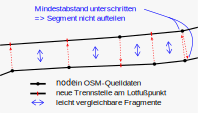
\includegraphics[width=\ScaleIfNeeded]{../chapter4/comparable-fragments}
    \caption{comparable-fragments}\label{fig:comparable-fragments}
\end{figure}



\section{Operationen}

Der zuvor beschriebene Lösungsansatz lässt sich vereinfacht als Sequenz von vier Operationen ausdrücken:\\
1. Segmente unterteilen\\
2. Analysieren\\
3. Punktezuordnung\\
4. Parallelen zusammenfassen\\

% Datenflussdiagramm

Die folgenden Abschnitte beschreiben jede dieser Operationen im Detail.

% Zur Vereinfachung Vorbedingungen der Eingabedaten: ...

% Definitionen: Ways haben Nodes; Segmente haben exakt zwei Nodes, welche mit folgender "Funktion zu erhalten sind; ...


\subsection{Segmente unterteilen}
\label{ch:split-algorithm}

In \osm-Daten sind seit Oktober~2007 Segmente (Verbindungen von exakt zwei \term{nodes}) nicht mehr als eigene Objekte enthalten \cf[57]{RT09}.
Anhand der aus der Datenquelle eingelesenen Menge aller \term{ways} wird daher zunächst durch \textproc{Segmentierung} die Menge aller Segmente ermittelt.

\begin{algorithm}[H]
\caption{Segmentierung}\label{alg:Segmentierung}
\begin{algorithmic}
\Function{Segmentierung}{$W$}\Comment{Menge aller \term{ways} $W$}
	\State $S \gets \varnothing$
	\ForAll{$w \textbf{ mit } w \in W $}
%		\State $N \gets$ alle \term{nodes} von $w$
%		\ForAll{$i \textbf{ mit } i \in \mathbb{N} : 0 < i < |N| $}\Comment{alle \term{nodes} außer dem ersten}
%			\State $n \gets$ \term{node} $i$ aus $N$
%			\State \textbf{füge} neues Segment ... \textbf{zu} $S$ \textbf{hinzu}
%		\ForAll{$n$ \textbf{mit} $n \in N \wedge \exists$ $m : m$ ist Vorgänger von $n$}
		\ForAll{$n$ \textbf{mit} $n \in w.nodes \wedge \exists$ $m : m$ ist Vorgänger von $n$ in $w$}
%			\State \textbf{füge} neues Segment $(m, n)$ \textbf{zu} $S$ \textbf{hinzu}
			\State $S \gets S \cup \{(m,n)\}$\Comment{neues Segment $(m, n)$ zu $S$ hinzufügen}
		\EndFor
	\EndFor
	\State \textbf{Ergebnis} $S$
\EndFunction
\end{algorithmic}
\end{algorithm}

Die Segmente werden anschließend durch \textproc{Splitten} derart aufgeteilt, dass ein geometrischer Vergleich leicht möglich wird (Abbildung~\ref{fig:comparable-fragments}).
Die so zerteilten Fragmente sind keine Segmente im Sinne der früheren gleichnamigen \osm-Objekte, da der Punkt, an dem sie zerteilt wurden, keinen \term{node} in OpenStreetMap darstellt.
Im Folgenden werden sie dennoch vereinfachend als Segmente bezeichnet.

Aufgeteilt werden Segmente jeweils am \textproc{Fußpunkt} eines Lots, das von einem \term{node} eines anderen Segments gefällt wird.
Der gewählte Algorithmus für das \textproc{Splitten} arbeitet geometrisch rekursiv:
Alle erzeugten Fragmente werden wieder zur Menge der Segmente hinzugefügt und somit immer weiter aufgeteilt, bis kein \textproc{Fußpunkt} mehr gefunden wird.

\begin{algorithm}[H]
\caption{Splitten}\label{alg:Splitten}
\begin{algorithmic}
\Function{Splitten}{$S$}\Comment{Menge aller Segmente $S$}
	\ForAll{$s \textbf{ mit } s \in S$}
		\ForAll{$n \textbf{ mit } n \in \{\textproc{Start}(s), \textproc{Ende}(s)\} $}
			\State $T \gets \textproc{NaheSegmente}(s, S)$
			\ForAll{$t \textbf{ mit } t \in T \wedge \exists$ $p_F : p_F = \textproc{Fußpunkt}(n, t)$}
				\State $t_1 \gets (\textproc{Start}(t), p_F)$
				\State $t_2 \gets (p_F, \textproc{Ende}(t))$
				\State $S \gets \{t_1, t_2\} \cup S \setminus \{t\}$
			\EndFor
		\EndFor
	\EndFor
	\State \textbf{Ergebnis} $S$
\EndFunction
\end{algorithmic}
\end{algorithm}

Um Verbindungen zwischen zwei \term{nodes} deterministisch beschreiben zu können, werden diese hier als Kanten in einem gerichteten Graphen betrachtet.
Dies betrifft sowohl alle Segmente als auch die später behandelten Punktezuordnungen (Abschnitt~\ref{ch:correlation-algorithm}).
Die beiden \term{nodes} werden als \textproc{Start} und \textproc{Ende} bezeichnet.

Geometrisch betrachtet entsprechen \term{nodes} Punkten, die durch vom Koordinatenursprung ausgehende Vektoren in der euklidischen Ebene definiert sind.
Segmente als gerichtete Verbindungen zweier solcher Punkte lassen sich dann ebenfalls als Vektoren auffassen und als geordnetes Paar notieren.

So könnten beispielsweise die Punkte $a$ und $b$ das Segment $(a,b)$ definieren, welches geometrisch dem Vektor $b - a$ entspräche.

% TODO: reicht hier schon die Prosa?

\begin{algorithm}[H]
\caption{Start / Ende}\label{alg:StartEnde}
\begin{algorithmic}
\Function{Start}{$s =: (n_1, n_2)$}
	\State \textbf{Ergebnis} $n_1$
\EndFunction
\Function{Ende}{$s =: (n_1, n_2)$}
	\State \textbf{Ergebnis} $n_2$
\EndFunction
\end{algorithmic}
\end{algorithm}

Es ist nicht notwendig, jedes Segment mit allen anderen Segmenten zu vergleichen.
Segmente, die zu weit entfernt und somit nicht \textproc{NaheSegmente} sind, können von vornherein als potenzielle Parallelen ausgeschlossen werden.
Zur Entscheidung, welche Segmente als „nah“ gelten und damit für Parallelität in Frage kommen, wird für jedes Segment eine \textproc{Hülle} gebildet, welche etwas größer als das jeweilige Segment ist, so dass sich die Hüllen von nahe beieinander liegenden Segmenten überschneiden.
% TODO: Grafik und/oder Literaturverweis

%Nachdem die \osm-Eingangsdaten für die Generalisierung vollständig bekannt und somit statisch sind, bietet sich hierzu der Einsatz eines gepackten R-Baums an \cf[255-256]{RSV02}.

%2. Regionalisierung
%- ∀ Segmente : Liste der "nahen" anderen Segmente
%→ Spatial Index / Array (sortiert)

\begin{algorithm}[H]
\caption{nahe Segmente}\label{alg:NaheSegmente}
\begin{algorithmic}
\Function{NaheSegmente}{$s, S$}\Comment{Menge aller Segmente $S$}
	\State \textbf{Ergebnis} $\{t : t \in S \wedge \textproc{Hülle}(s) \cap \textproc{Hülle}(t) \neq \varnothing\}$
\EndFunction
\end{algorithmic}
\end{algorithm}

Als \textproc{Hülle} könnte ein Puffer dienen.
Aus Gründen der Effizienz bietet es sich jedoch an, die \textproc{Hülle} rechteckig im Koordinatennetz anzulegen.
Für diesen Fall hängt die Größe der Hülle auch von der Orientierung des Segments ab.
Im Ergebnis wird später zu sehen sein, dass diagonal zum Koordinatennetz ausgerichtete Segmente bei größeren Abständen zueinander als parallel erkannt werden als solche Segmente, die orthogonal zum Koordinatennetz ausgerichtet sind.

Weiterhin hängen diese Erkennungsabstände vom gewählten Koordinatennetz ab.
Wird beispielsweise mit geographischen Koordinaten gearbeitet, variiert das Verhältnis der Erkennungsabstände in Ost/West- und in Nord/Süd-Richtung mit der geographischen Breite.
Insbesondere auf höheren Breiten bietet sich daher der Einsatz einer winkeltreuen Abbildung wie etwa Gauß-Krüger an, um diese Einflüsse zu minimieren.
Für die Korrektheit der Algorithmen spielen beide Arten von Variationen jedoch keine Rolle, solange die Erkennungsabstände nicht fest vorgegeben sind.
% TODO: Grafik?

\begin{algorithm}[H]
\caption{Definition der erweiterten Hüllfunktion für \textproc{NaheSegmente}}\label{alg:Huelle}
\begin{algorithmic}
\Function{Hülle}{$s$}
	\State \textbf{Ergebnis} sei die nach allen Kardinalrichtungen um $\eta/2$ vergrößerte rechteckige Hülle um das Segment $s$, wobei $\eta$ der festzulegende Höchstabstand sei, für den zwei Segmente als „nahe“ gelten dürfen.
\EndFunction
\end{algorithmic}
\end{algorithm}

%3. Orientierungs-Ausschluss
%- ∀ Segmente : Liste der "nahen und geometrisch parallelen" Segmente

%, die weder zu weit entfernt sind noch deren Ausrichtung zu sehr abweicht.

%...

%4. Splitten ("re-entrant") in Fragmente
%Liste B aller `LinePart` als Basis (initial: alle `LineSegment`)
%- _∀ B : P₁, P₂_
%    - _∀ P_ als p
%        - _∀ `splitTargets()`_ : (_target noch nicht gesplittet_ -> next;)
%            - Fußpunkt PF für p auf target suchen
%            - falls nicht außerhalb target (✐) / falls ≠ target.P₁, target.P₂: *Split* target bei PF
%                - neue Fragmente f₁, f₂ mit P₁–PF und PF–P₂ erzeugen
%                - beide f₁, f₂ an Controller melden (für Basis-Iterator: hinten anhängen an Liste zu splittender Segmente)
%                - Basis und target als gesplittet / "fertig" markieren
%                - … mehr an Controller melden…?
%(`splitTargets()`: Liste der "nahen" anderen Segmente)

Das Aufteilen in Fragmente erfolgt jeweils am \textproc{Fußpunkt}~(Abbildung~\ref{fig:footpoint}).

\begin{algorithm}[H]
\caption{Fußpunkt}\label{alg:Fusspunkt}
\begin{algorithmic}
\Function{Fußpunkt}{$n,t$}
%	\State Es sei $l \bot t$ und $n \in l$. Dann sei $f \coloneq l \cap t$ bei $min(||f-t_1||, ||f-t_2||) > \varepsilon$ $\wedge$ $max(||f-t_1||, ||f-t_2||) < ||t||$, wobei $\varepsilon$ die festzulegende Mindestlänge eines Fragments sei.
	\State \textbf{Ergebnis} sei der Lotfußpunkt~$f$ des Punkts~$n$ auf der Geraden~$t$. Liegt~$f$ nicht zwischen den Punkten $\textproc{Start}(t)$ und $\textproc{Ende}(t)$ oder liegt~$f$ näher an $\textproc{Start}(t)$ oder $\textproc{Ende}(t)$ als die festzulegende Mindestlänge~$\mu$ eines Fragments, dann gibt es kein Ergebnis.
% Der zweite Satz ist ein wesentliches, aber nicht unbedingt offensichtliches Detail, deshalb sollte auch das an sich einfache Konzept "Lotfußpunkt" formal beschrieben werden.
\EndFunction
\end{algorithmic}
\end{algorithm}

\begin{figure}[ht]
    \centering
    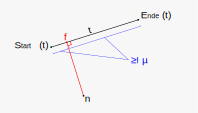
\includegraphics[width=\ScaleIfNeeded]{../chapter4/footpoint}
    \caption{footpoint}\label{fig:footpoint}
\end{figure}

\subsection{Analysieren}
\label{ch:analyse-algorithm}

Das Ergebnis der Operation „Segmente unterteilen“ eignet sich zur \textproc{Analyse} auf Parallelität.
Hierfür werden Geometrie und Attribute näher verglichen.
Für jedes Segment wird beidseitig jeweils genau ein anderes Segment als parallel gekennzeichnet, sofern auf der jeweiligen Seite wenigstens ein nahes paralleles Segment existiert.

Die Unterscheidung der Seiten links und rechts erfolgt durch Bestimmung der Winkel zu den \term{nodes} des jeweils anderen Segments.

%5. Analyse der Fragmente
%∀ Fragmente:
%- Ähnlichkeitsmaß zu allen anderen in Frage kommenden Fragmenten bestimmen (⇐ `closeParallels`), sortieren
%- aussortieren über `Analyser`
%- ∀ verbleibenden anderen Fragmente: best match(es) L+R finden, falls vorhanden (teilen 2 Segmente einen Node, ist es kein Match! (sonst klappt die L/R-Punktfindung nicht richtig)
%- best match(es) für _Segmente_ eintragen in eine Liste (und zwar reziprok) (→ eigentlich unnötig??) (∀ Segmente: ∃ 2 Listen "paralleler" Segmente) L+R (|||)

...

\begin{algorithm}[H]
\caption{Analyse}\label{alg:Analyse}
\begin{algorithmic}
\State $\textbf{Variable } parallelLinks : Segment \rightarrow Segment$
\State $\textbf{Anfangswert } parallelLinks(a) \stackrel{\text{\tiny def}}{=} \varnothing$ $\forall$ $a$
\State $\textbf{Variable } parallelRechts : Segment \rightarrow Segment$
\State $\textbf{Anfangswert } parallelRechts(a) \stackrel{\text{\tiny def}}{=} \varnothing$ $\forall$ $a$
\Function{Analyse}{$S$}
	\ForAll{$s \textbf{ mit } s \in S$}
		\State $T \gets \{t : t \in \textproc{NaheSegmente}(s, S) \wedge \textproc{Parallel}(s, t)\}$
		\State $L \gets \{t : t \in T \wedge \sphericalangle (s, \textproc{Start}(t) - \textproc{Start}(s)) < 0 \wedge \sphericalangle (s, \textproc{Ende}(t) - \textproc{Start}(s)) < 0\}$
		\State $R \gets \{t : t \in T \wedge \sphericalangle (s, \textproc{Start}(t)  - \textproc{Start}(s)) > 0 \wedge \sphericalangle (s, \textproc{Ende}(t) - \textproc{Start}(s)) > 0\}$
		\State\Comment{Winkel seien definiert im Intervall $(-\pi,\pi)$ und im Uhrzeigersinn}
		\ForAll{$l \textbf{ mit } l \in L$}\Comment{Menge $L$ aller nahen Parallelen linksseitig}
			\State $parallelLinks(s) \gets l \textbf{ falls } 0 < \textproc{Distanz}(s, l) \leqslant \textproc{Distanz}(s, l')$ $\forall$ $l' \in L$
		\EndFor
		\ForAll{$r \textbf{ mit } r \in R$}\Comment{Menge $R$ aller nahen Parallelen rechtsseitig}
			\State $parallelRechts(s) \gets r \textbf{ falls } 0 < \textproc{Distanz}(s, r) \leqslant \textproc{Distanz}(s, r')$ $\forall$ $r' \in R$
		\EndFor
	\EndFor
	\State \textbf{Ergebnis} $parallelLinks, parallelRechts$
\EndFunction
\end{algorithmic}
\end{algorithm}

\begin{algorithm}[H]
\caption{Parallel TBD}\label{alg:Parallel}
\begin{algorithmic}
\Function{Parallel}{$s_1, s_2$}
	\State Die Segmente $s_1$ und $s_2$ seien parallel genau dann, wenn sie ähnlich ausgerichtet sind (closeParallels-Winkel) und die für den speziellen Anwendungsfall festgelegten Bedingungen auf die zugehörigen OSM-Ways zutreffen (Analyser-Bedingungen: shouldEvaluate und evaluate); siehe Kapitel 3 (TBD).
	\State (dazu gehörend auch maximale Distanz $\zeta$)
\EndFunction
\end{algorithmic}
\end{algorithm}

Aus der Menge aller parallelen Segmente auf einer Seite wird dasjenige mit der kürzesten \textproc{Distanz} als Parallele ausgewählt.
Auf welche Weise die Distanz zwischen zwei Segmenten bestimmt wird, kann vom speziellen Anwendungsfall abhängen und soll hier nicht definiert werden.

% tatsächlich implementiert: Summe der Abstände der jeweils nächsten Nodes (siehe MyAnalyser.evaluate)
% alternativ denkbar: _kleinster_ Abstand zweier Nodes

\begin{algorithm}[H]
\caption{Beispielhafte Bestimmung der Distanz zweier Segmente}\label{alg:Distanz}
\begin{algorithmic}
\Function{Distanz}{$s_1, s_2$}
	\State \textbf{Ergebnis} $ $ % TODO: Distanz der Mittelpunkte
	\State Distanz der Segmente $s_1$ und $s_2$ z. B. einfach die Summer der Distanz der jeweils nächsten Endpunkte (siehe MyAnalyser.evaluate) oder die Distanz der Mittelpunkte (evtl. einfacher zu definieren) – TBD.
\EndFunction
\end{algorithmic}
\end{algorithm}

\begin{algorithm}[H]
\caption{Mittelpunkt}\label{alg:Mittelpunkt}
\begin{algorithmic}
\Function{Mittelpunkt}{$a$}
	\State \textbf{Ergebnis} $\frac{\textproc{Start}(a) + \textproc{Ende}(a)}{2}$
\EndFunction
\end{algorithmic}
\end{algorithm}

%6. Links/Rechts filtern
%(Albaufstieg vs. Verteilerfahrbahnen)
%
%_defer_
%
%Basis: Vergleichsfaktor  
%z. B. _R_ ignorieren, falls Distanz zu _R_ *m*-fach Distanz zu _L_ ist (*m* ≈ 2,5)

...


\subsection{Punktezuordnung}
\label{ch:correlation-algorithm}

%7. Punktzuordnungen erzeugen (Vorstufe Generalisierung)
%
%- ∀ Segmente "S" : S hat Parallele und S noch nicht "fertig 7"
%    - ∀ Punkte (Start/End "T₁"), ∀ Seiten von S (L/R) "A"
%        - ∀ Parallelen von S "P" auf Seite A
%            - nahegelehensten Punkt finden "T₂"
%            - falls nichts gefunden (= keine Parallele auf dieser Seite), näcshtes A
%            - neue Punktzuordung: T₁ ↔︎ T₂
%    - S markieren als "fertig 7"
%
%_defer:_
%- ∀ Parallelen von S: Rekursion
%- alle Segmente/Zuordnungen für je ein ursprüngliches Segment als Teil eines "Blocks" markieren (könnte später evtl. Auffinden eines Anfangs zur Generalisierung erleichtern)

...

\begin{algorithm}[H]
\caption{Nodes Zuordnen}\label{alg:Zuordnen}
%$\textbf{Variable } fertig7 : Segment \rightarrow bool$
%\\$\textbf{Anfangswert } fertig7(a) \stackrel{\text{\tiny def}}{=} nein$ $\forall$ $a$
\begin{algorithmic}
\Function{NodesZuordnen}{$S$}
	\State $C \gets \varnothing$
	\ForAll{$s \textbf{ mit } s \in S$}% \wedge \neg$ $fertig7(t)$}
		\ForAll{$t \textbf{ mit } t \in \{parallelLinks(s), parallelRechts(s)\}$}
			\ForAll{$n_1 \textbf{ mit } n_1 \in \{\textproc{Start}(s), \textproc{Ende}(s)\} $}
				\State $n_2 \gets \begin{cases}\textproc{Start}(t) & \text{für } ||n_1 - \textproc{Start}(t)|| < ||n_1 - \textproc{Ende}(t)||\\\textproc{Ende}(t) & \text{sonst}\end{cases}$
				\State $C \gets C \cup (n_1, n_2)$\Comment{$n_2$ ist der $n_1$ am nächsten gelegene \term{node} von $t$}
			\EndFor
		\EndFor
%		\State $fertig7(s) \gets ja$
	\EndFor
	\State \textbf{Ergebnis} $C$
\EndFunction
\end{algorithmic}
\end{algorithm}


\subsection{Parallelen zusammenfassen}
\label{ch:generalisation-algorithm}

%8. Generalisierung
%
%"trivialer Fall":
%1. zufällig Segment S wählen, Edge E (ES, ET) (Bedingung: Zähler E < 2)
%2. Richtung D zufällig wählen (-> S); {F,R}
%    1. gegenüberliegendes Segment T (für Start): dasjenige der beiden (<- trivialer Fall) Segment von ET, welches -- so gedreht, dass der Start-Node == ES ist -- in die gleiche Richtung zeigt wie S
%3. ∀ D :
%    1. wiederhole, solange ∃ E
%4. M-Punkt setzen
%    5. Segmente A,B von E in Richtung D: nächste Nodes N {X,Y} finden (falls ∄: N:= aktueller Node
%    6. ∀ N:
%        7. Edge F von N zurück zu E? (X->ET, Y->ES)
%           ∃: F ist nächstes E; Zähler E + 1, Zähler F + 1
%           ∄: continue 6, sonst: Edge F(X,Y)
%              ∃: F ist nächstes E
%      E=F <=> ∄: Zähler E + 1, continue 3

...

Diese Beschreibung des Algorithmus zum \textproc{Zusammenfassen} bildet der Übersichtlichkeit halber nur den trivialen Fall ab, dass es keine Kreuzungen gibt und dass es für jede Zusammenfassung genau zwei Segmente gibt, die durch sie wegfallen.

% TODO: dies scheint mit Segments, nicht mit Fragments zu laufen -- prüfen, ob das hier richtig abgebildet wird

\begin{algorithm}[H]
\caption{Zusammenfassen}\label{alg:Zusammenfassen}
\begin{algorithmic}
\Function{Zusammenfassen}{$S, C$}
	\State generalisierter Graph $\mathcal{G} \gets$ leer
	\ForAll{Segmente $s$, die noch nicht als zusammengefasst markiert sind}
		\ForAll{Zuordnungen $e$, die mit dem Start-Node $n$ von $s$ verknüpft sind}
			\State zusammengefasster Linienzug $L \gets$ leer
			\State $t \gets$ mit dem jeweils anderem Node von $e$ verknüpftes Segment, welches von $n$ aus gesehen in die gleiche Richtung zeigt wie $s$
			\While{es eine nächste Zuordnung $f$ gibt, die $s$ und $t$ an deren anderen Ende ebenfalls einander zuordnet}
				\State $m \gets$ Mittelpunkt von $e$
				\State $m' \gets$ Mittelpunkt von $f$
				\State füge Segment $(m, m')$ zu $L$ hinzu
				\State markiere $s$ und $t$ als zusammengefasst
				\State $s \gets$ Segment, das $s$ nach $f$ fortführt
				\State $t \gets$ Segment, das $t$ nach $f$ fortführt
			\EndWhile
			\State füge $L$ zu $\mathcal{G}$ hinzu
		\EndFor
	\EndFor
	\State füge alle nicht zusammengefassten Segmente zu $\mathcal{G}$ hinzu
	\State \textbf{Ergebnis} $\mathcal{G}$
\EndFunction
\end{algorithmic}
\end{algorithm}


% mit vorwärts/rückwärts-Logik (nur sinnvoll, wenn man das Verketten für Wesentlich hält, was das Themenblatt nicht tut ("Verkettung, soweit zum Zusammenfassen nötig")
%\begin{algorithm}[H]
%\caption{Zusammenfassen}\label{alg:Zusammenfassen}
%\begin{algorithmic}
%\Function{Zusammenfassen}{$S, C$}
%	\State generalisierter Graph $\mathcal{G} \gets$ leer
%	\ForAll{Segmente $s$, die noch nicht als zusammengefasst markiert sind}
%		\ForAll{Zuordnungen $e$, die mit dem Start-Node $n$ von $s$ verknüpft sind}
%			\State zusammengefasster Linienzug $L \gets$ leer
%			\State $t \gets$ mit dem jeweils anderem Node von $e$ verknüpftes Segment, welches von $n$ aus gesehen in die gleiche Richtung zeigt wie $s$
%			\While{es eine nächste Zuordnung $f$ gibt, die $s$ und $t$ an deren anderen Ende ebenfalls einander zuordnet}
%				\State $m \gets$ Mittelpunkt von $e$
%				\State $m' \gets$ Mittelpunkt von $f$
%				\State füge Segment $(m, m')$ am Ende von $L$ hinzu
%				\State markiere $s$ und $t$ als zusammengefasst
%				\State $s \gets$ Segment, das $s$ nach $f$ fortführt
%				\State $t \gets$ Segment, das $t$ nach $f$ fortführt
%			\EndWhile
%			\State $s \gets$ Segment, das $s$ in die Gegenrichtung fortführt
%			\State $t \gets$ mit dem jeweils anderem Node von $e$ verknüpftes Segment, welches von $n$ aus gesehen in die gleiche Richtung zeigt wie $s$
%			\While{es eine nächste Zuordnung $f$ gibt, die $s$ und $t$ an deren anderen Ende ebenfalls einander zuordnet}
%				\State $m \gets$ Mittelpunkt von $e$
%				\State $m' \gets$ Mittelpunkt von $f$
%				\State füge Segment $(m, m')$ am Anfang von $L$ hinzu
%				\State markiere $s$ und $t$ als zusammengefasst
%				\State $s \gets$ Segment, das $s$ nach $f$ fortführt
%				\State $t \gets$ Segment, das $t$ nach $f$ fortführt
%			\EndWhile
%			\State füge $L$ zu $\mathcal{G}$ hinzu
%		\EndFor
%	\EndFor
%	\State füge alle nicht zusammengefassten Segmente zu $\mathcal{G}$ hinzu
%	\State \textbf{Ergebnis} $\mathcal{G}$
%\EndFunction
%\end{algorithmic}
%\end{algorithm}

% Versuche mit Formelsatz
%\begin{algorithm}[H]
%\caption{Zusammenfassen}\label{alg:Zusammenfassen}
%%$\textbf{Variable } zusammengefasst : Segment \rightarrow bool$
%%\\$\textbf{Anfangswert } zusammengefasst(a) \stackrel{\text{\tiny def}}{=} nein$ $\forall$ $a$
%% \neg$ $zusammengefasst(s)
%\begin{algorithmic}
%\Function{Zusammenfassen}{$S, C$}
%	\ForAll{$s \textbf{ mit } s \in S, s =: (n_1, n_2)$}
%		\ForAll{$e \textbf{ mit } e \in C, e =: (e_1, e_2) \wedge (e_1 = n_1 \vee e_2 = n_1)$}
%			\State $T \gets \{t : t \in S, t =: (n_3, n_4) \wedge |\{e_1, e_2, n_3, n_4\}| < 4\}$
%			% T <- alle Segmente von ET
%			\ForAll{$t \textbf{ mit } t \in T, t =: (n_3, n_4)$}
%				
%				\State $ $ % hierhin jetzt die "cases" für die Drehung/Unterscheidung, damit bei 2.->1. das richtige ES/ET kommt
%			% ^--- "in die gleiche Richtung zeigt wie S" - wie ist das gemeint?
%				
%				
%			\EndFor
%		\EndFor
%	\EndFor
%	
%	
%%	\State $C \gets \varnothing$
%%	\ForAll{$s \textbf{ mit } s \in S, s =: (n_1, n_2)$}% \wedge \neg$ $fertig7(t)$}
%%		\ForAll{$t \textbf{ mit } t \in \{parallelLinks(s), parallelRechts(s)\}, t =: (n_3, n_4)$}
%%			\ForAll{$e_1 \textbf{ mit } e_1 \in \{n_1, n_2\} $}
%%				\State $e_2 \gets \begin{cases}n_3 & \text{für } ||e_1 - n_3|| \textless ||e_1 - n_4||\\n_4 & \text{sonst}\end{cases}$
%%				\State $C \gets C \cup (e_1, e_2)$\Comment{$e_2$ ist der $e_1$ am nächsten gelegene \term{node} von $t$}
%%			\EndFor
%%		\EndFor
%%%		\State $fertig7(s) \gets ja$
%%	\EndFor
%%	\State \textbf{Ergebnis} $C$
%\EndFunction
%\end{algorithmic}
%\end{algorithm}


\section{Gesamtüberblick}

\begin{algorithm}[H]
\caption{Generalisierung}\label{alg:Generalisierung}
\begin{algorithmic}
\Function{Generalisierung}{$W$}
	\State $S \gets \textproc{Splitten}(\textproc{Segmentierung}(W))$\Comment{Segmente unterteilen, Abschnitt~\ref{ch:split-algorithm}}
	\State $\textproc{Analyse}(S)$\Comment{auf Parallelität analysieren, Abschnitt~\ref{ch:analyse-algorithm}}
	\State $C \gets \textproc{NodesZuordnen}(S)$\Comment{Generalisierung vorbereiten, Abschnitt~\ref{ch:correlation-algorithm}}
	\State $\mathcal{G} \gets \textproc{Zusammenfassen}(S, C)$\Comment{Generalisierung durchführen, Abschnitt~\ref{ch:generalisation-algorithm}}
	\State \textbf{Ergebnis} $\mathcal{G}$
\EndFunction
\end{algorithmic}
\end{algorithm}


\section{alte Einteilung}

\subsection{Identifikation parallel verlaufender Linien-Fragmente}

Ansatz: Dieser Algorithmus eignet sich insgesamt weniger gut zur Identifikation als zur Generalisierung.
Die Identifikation erfolgt, indem festgestellt wird, ob eine Generalisierung notwendig ist oder nicht; falls sie notwendig ist, kann sie dann aber auch bereits recht billig durchgeführt werden.
Andererseits ist fraglich, welchen "praxistauglichen" Einsatz eine reine Identifikation ohne anschließende Generalisierung hätte.

Konzept (abstrakt):

1. nur Segmente betrachten (gerade Linienabschnitte, definiert durch zwei Punkte)

2. alle nahe beieinander liegenden Segmente auf Parallelität untersuchen

Die Segmente sind jedoch unterschiedlich lang und liegen teilweise etwas „verstreut“ im Raum, was die Untersuchung erschwert.
Deshalb werden die Segmente zunächst fragmentiert, indem benachbarte Segmente „geschickt“ weiter in kürzere Segmente unterteilt werden, so dass parallele Segmente immer ähnlich lang sind und einander gegenüberstehen.

Im Detail:

1. geometrische Indizierung (R-Tree) der Eingabedaten, um Suche nach nahen LineParts zu ermöglichen [regionalise]

2. $\forall$ LineParts: AbstractLinePart.splitCloseParallels, um gut vergleichbare Stücke zu erhalten (reentrant/rekursiv, d. h. neu erzeugte Fragmente werden bis zu einer Mindestgröße immer weiter aufgeteilt) [split]

3. $\forall$ LineParts: $\forall$ nahe Parallelen (laut Index): [analyse]

3.1 Vorprüfung (boolean)

3.2 Hauptprüfung (double)

3.3 best matches (links/rechts getrennt) speichern (keine Nachprüfung => falls das best match nicht passt, wird es trotzdem genommen, sofern nicht schon die vorprüfung die sache abgebrochen hat)
% offen: "realParallels"-Konzept
% geprüft werden die Fragmente, gespeichert werden die Segmente

% graphisch erklären, was genau passiert


\subsection{Generalisierung durch Zusammenfassung}

Konzept (in den allgemeinsten Begriffen):

1. Endpunkte der parallelen Segmente einander zuordnen

2. Der gesamte Graph wird "durchgehangelt", indem von einer CorrelationEdge ausgehend immer entlang der Segmente das nächste CorrelationEdge gefunden wird; diese Edges werden dann durch neu erzeugte Mittelpunkte miteinander verbunden.



% (Der CorrelationGraph ist ein Graph, in dem CorrelationEdges einander gegenüberliegende Knoten von parallelen Segmenten verbinden.)

% new GeneralisedLines
% - beliebige CorrelationEdge auswählen und von ihr ausgehend den angrenzenden Segmenten erst in die eine, dann die andere Richtung folgen, bis das Folgen nicht mehr eindeutig möglich ist (z. B. wegen einer Abzweigung)
% - dabei Mittelpunkte der CorrelationEdges jeweils einer neuen GeneralisedSection hinzufügen
% - Segmente, die nicht zusammengefasst wurden (weil keine Parallelen existieren), werden in Sections umgewandelt und ebenfalls den GeneralisedLines hinzugefügt, um einen homogenen Ergebnisdatensatz zu erhalten

...


\subsection{Verknüpfung von Linienfragmenten zu einem einzigen kontinuierlichen Linienzug}

...


% single-chapter commands
%\onlyinsubfile{\listoffigures} \onlyinsubfile{\listoftables}
%\onlyinsubfile{% global bibliography settings

\nocite{*}  % include works in bibliography that aren't cited anywhere in the document (for debugging)

\setbibpreamble{Die Literaturangaben sind alphabetisch nach den Nachnamen der Autoren sortiert. Bei mehreren Autoren wird nach dem ersten Autor sortiert.\par\bigskip\bigskip}

\bibliography{../references-papers,../references-manual}
%\bibliography{../references-manual}
}
\end{document}
